\documentclass[aspectratio=169]{beamer}
\usetheme[numbering=fraction]{metropolis}

% ── Ruban titre ───────────────────────────────────────────────
\makeatletter
\setlength{\metropolis@frametitle@padding}{1ex}
\makeatother

% ── Suppression des slides de transition de section ──────────
\metroset{sectionpage=none}

\usepackage[french]{babel}
\usepackage[T1]{fontenc}
\usepackage[utf8]{inputenc}
\usepackage{lmodern}
\usepackage{csquotes}
\usepackage{xcolor}
\usepackage{graphicx}
\usepackage{booktabs}
\usepackage{caption}
\usepackage{tikz}
\usetikzlibrary{arrows.meta,positioning,calc,decorations.pathmorphing}
\usepackage{varwidth}
\usepackage{colortbl}
\usepackage{array}
\usepackage{amsmath}
\usepackage{appendixnumberbeamer}
\graphicspath{{../../../results/morvan/figures/}{../../../results/figures/}{./}}

% ================================================================
% COULEURS
% ================================================================
\definecolor{myblue}{HTML}{1F4E79}
\definecolor{myblue2}{HTML}{2E6BA8}
\definecolor{myorange}{HTML}{E07B39}
\definecolor{mygreen}{HTML}{2E7D32}
\definecolor{myred}{HTML}{C0392B}
\definecolor{myteal}{HTML}{006064}
\definecolor{mylgray}{HTML}{F4F6F9}
\definecolor{mymgray}{HTML}{D0D8E4}
\definecolor{mydgray}{HTML}{4A5568}
% bandes radar (mêmes couleurs que les figures)
\definecolor{Lband}{HTML}{2E7D32}
\definecolor{Cband}{HTML}{7B4FA8}
\definecolor{cut}{HTML}{C0392B}
\definecolor{ctrl}{HTML}{1F77B4}

% ================================================================
% COULEURS BEAMER
% ================================================================
\setbeamercolor{frametitle}{bg=myblue, fg=white}
\setbeamercolor{progress bar}{fg=myblue, bg=gray!20}
\setbeamercolor{block title}{bg=myblue, fg=white}
\setbeamercolor{block body}{bg=mylgray}
\setbeamercolor{block title alerted}{bg=myorange, fg=white}
\setbeamercolor{block body alerted}{bg=mylgray}
\setbeamercolor{block title example}{bg=mygreen, fg=white}
\setbeamercolor{block body example}{bg=mylgray}
\setbeamercolor{alerted text}{fg=myorange}
\setbeamercolor{bibliography entry author}{fg=myblue}
\setbeamercolor{bibliography entry title}{fg=myblue}

\captionsetup{labelfont=bf, font=small}

\newcommand{\Lb}[1]{\textcolor{Lband}{\textbf{#1}}}
\newcommand{\Cb}[1]{\textcolor{Cband}{\textbf{#1}}}

% ================================================================
% COMMANDE SOUS-TITRE DE SLIDE
% ================================================================
\newcommand{\slidesubtitle}[1]{%
	\textcolor{myblue}{\small\textbf{#1}}%
	\par\vspace{3pt}%
}
% chiffre clé : couleur, valeur, légende
\newcommand{\keynum}[3]{%
	\begin{minipage}[t]{0.31\linewidth}\centering
		\textcolor{#1}{\Large\textbf{#2}}\\[1pt]
		\scriptsize #3
	\end{minipage}}

% ================================================================
% BIBLIOGRAPHIE
% ================================================================
\usepackage[backend=biber, style=authoryear,
maxcitenames=2, mincitenames=1,
isbn=false, eprint=false, doi=false, url=false]{biblatex}
\addbibresource{../../latex/references.bib}

\AtBeginDocument{%
	\renewcommand*{\mkbibnamefamily}[1]{\textnormal{#1}}%
	\renewcommand*{\mkbibnamegiven}[1]{\textnormal{#1}}%
	\renewcommand*{\mkbibnameprefix}[1]{\textnormal{#1}}%
	\renewcommand*{\mkbibnamesuffix}[1]{\textnormal{#1}}%
}
\DeclareCiteCommand{\parencite}
{\usebibmacro{prenote}}
{\textcolor{black}{(}\textcolor{myred}{\usebibmacro{cite}}\textcolor{black}{)}}
{\multicitedelim}
{\usebibmacro{postnote}}

% ================================================================
% PIED DE PAGE
% ================================================================
\setbeamercolor{footline}{bg=white, fg=black}
\setbeamerfont{footline}{size=\scriptsize}
\setbeamertemplate{footline}{%
	\hbox{%
		\begin{beamercolorbox}[wd=\paperwidth, ht=1.5ex,
			dp=0.6ex, leftskip=0.4cm,
			rightskip=0.4cm]{footline}
			\color{black}\rule{\paperwidth}{0.3pt}\par
			\vspace{-0.25em}
			\hfill \insertframenumber/\inserttotalframenumber
		\end{beamercolorbox}%
	}%
}

% ================================================================
% PAGE DE TITRE PERSONNALISEE
% ================================================================
\setbeamertemplate{title page}{%
	\begin{tikzpicture}[overlay, remember picture]
		\node[anchor=north west, xshift=0.5cm, yshift=-0.45cm]
		at (current page.north west)
		{
\includegraphics[height=0.9cm]{../../presentation/logos/logo_icube.png}};
		\node[anchor=north east, xshift=-0.5cm, yshift=-0.35cm]
		at (current page.north east)
		{
\includegraphics[height=1.3cm]{../../presentation/logos/logo_sertit.png}};
	\end{tikzpicture}%
	\vspace*{1.1cm}
	\vfill
	\begin{center}
		\footnotesize\textcolor{mydgray}{%
			Dossier de candidature -- Stage SERTIT / ICube (Université de Strasbourg)}

		\vspace{0.3em}
		\scriptsize\textcolor{mydgray}{%
			\og Exploration des bandes L et P (NISAR, BIOMASS) pour la détection de la déforestation
			et des glissements de terrain \fg}

		\vspace{0.9em}

		\begin{varwidth}{0.92\linewidth}
			\centering
			{\usebeamerfont{title}\usebeamercolor[fg]{title}%
				\inserttitle\par}
		\end{varwidth}

		\vspace{0.6cm}

		{\usebeamerfont{author}\usebeamercolor[fg]{author}%
			\insertauthor\par}

		\vspace{0.4cm}

		{\usebeamerfont{date}\usebeamercolor[fg]{date}%
			\insertdate\par}
	\end{center}
	\vfill
}

\title{\Large
	Bande L (NISAR) contre bande C (Sentinel-1)\\
	pour détecter les coupes rases dans le Morvan :\\[4pt]
	{\normalsize réplication selon la méthode du guide de l'Irstea}
}
\author{%
	Candidat : \textbf{Mamadou G. Diallo}
}
\date{Novembre 2026}

% ================================================================
\begin{document}

\begin{frame}
	\titlepage
\end{frame}

\begin{frame}{Plan}
	\tableofcontents
\end{frame}

% ================================================================
\section{Introduction}
% ================================================================

\begin{frame}{\phantom{x}}
	\frametitle{Introduction (1/2)}
	\vspace{-6pt}\scriptsize
	\begin{columns}[T]
		\column{0.52\textwidth}
		\begin{block}{Ce que les Vosges ont montré}
			\scriptsize
			\begin{itemize}
				\setlength{\itemsep}{0pt}
				\item Cohérence \Lb{L} : AUC \textbf{0,995} contre 0,74 en \Cb{C} sur la coupe C11
				\item Rétrodiffusion : avantage \Lb{L} en montante seulement
				\item \textcolor{myorange}{\textbf{Deux limites}} : \textbf{une seule coupe}, \textbf{une seule orbite}
				Sentinel-1
			\end{itemize}
		\end{block}
		\begin{block}{Objectifs de la réplication}
			\scriptsize
			\begin{enumerate}
				\setlength{\itemsep}{0pt}
				\item \textbf{Plusieurs coupes}, vérifiées une à une, \textbf{à géométrie égale}
				\item Une \textbf{méthode opérationnelle} française : le guide de l'Irstea \parencite{ose2015guide}
				\item Une chaîne transposable à \textbf{ROSE-L} \parencite{esa2020rosel} et aux produits \textbf{ISCE3}
				\parencite{isce3}
			\end{enumerate}
		\end{block}

		\column{0.44\textwidth}
		\begin{block}{Le guide de l'Irstea (2015)}
			\scriptsize
			\begin{itemize}
				\setlength{\itemsep}{0pt}
				\item Établi pour le ministère de l'Agriculture sur la sylvo-écorégion \textbf{G23
				\enquote{Morvan et Autunois}}
				\item $\Delta$NDVI dans la forêt, seuils $m-k\sigma$ : \textbf{degrés de certitude} 1, 2, 3
				\item Tamisage à 1~ha, matrice de confusion \textbf{en surface}
				\item Objectif : $\leq 10$~\% d'omission et de commission
			\end{itemize}
		\end{block}
		\vspace{2pt}
		\scriptsize Le guide sert deux fois : \textbf{référence optique} (sur Sentinel-2) et \textbf{norme
		d'évaluation} (transposé au radar).
	\end{columns}
\end{frame}

\begin{frame}{\phantom{x}}
	\frametitle{Introduction (2/2)}
	\slidesubtitle{Question et hypothèses (reprises des Vosges)}
	\begin{alertblock}{Question}
		\small Sur plusieurs coupes du Morvan (juin--novembre 2026), \textbf{à géométrie égale}, la bande \Lb{L}
		distingue-t-elle mieux les coupes que la bande \Cb{C} ? La méthode du guide est-elle transposable au radar ?
	\end{alertblock}
	\vspace{0.5em}
	\begin{block}{Hypothèses}
		\footnotesize
		\begin{itemize}
			\setlength{\itemsep}{3pt}
			\item[\textbf{H1}] Forêt intacte : cohérence plus élevée en \Lb{L} qu'en \Cb{C}
			\parencite{zebker1992decorrelation}.
			\item[\textbf{H2}] Donc une perte de cohérence due à la coupe mieux détectée en \Lb{L}.
			\item[\textbf{H3}] Une baisse de rétrodiffusion plus forte en \Lb{L}, la bande C saturant sur forêt dense
			\parencite{imhoff1995saturation,joshi2015mapping}.
			\item[\textbf{H4}] La polarisation croisée est l'indicateur de rétrodiffusion le plus sensible.
		\end{itemize}
	\end{block}
\end{frame}

% ================================================================
\section{Données et méthodologie}
% ================================================================

\begin{frame}{\phantom{x}}
	\frametitle{Données et méthodologie (1/3)}
	\slidesubtitle{1-Zone d'étude et données}
	\begin{columns}[c]
		\column{0.46\textwidth}
		\centering
		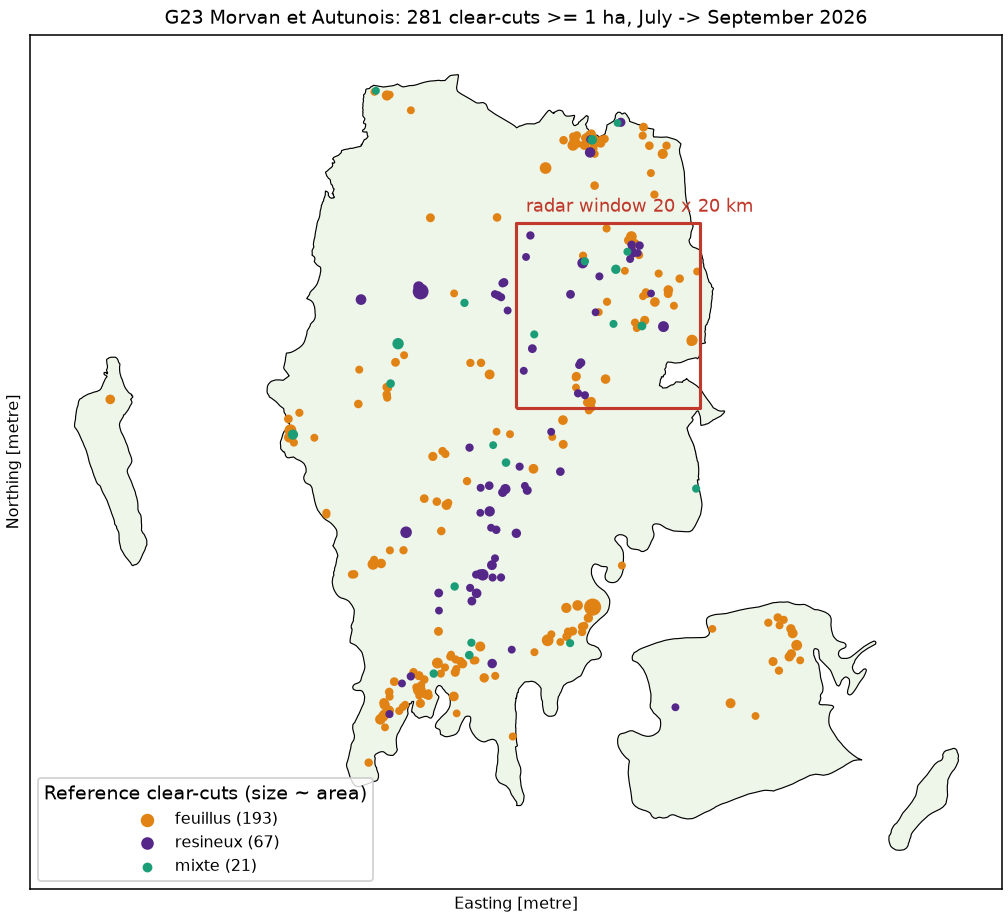
\includegraphics[width=\linewidth, height=0.68\textheight, keepaspectratio]{s2_reference_window.png}
		\captionof{figure}{Fenêtre radar de $20\times20$~km dans la G23.}

		\column{0.52\textwidth}
		\scriptsize
		\renewcommand{\arraystretch}{1.25}
		\begin{tabular}{|l|c|c|}
			\hline
			\rowcolor{myblue}\textcolor{white}{\textbf{Visée}} & \textcolor{white}{\textbf{Bande L (NISAR)}} &
			\textcolor{white}{\textbf{Bande C (S1)}} \\
			\hline
			Montante & \Lb{A173 F25} & \Cb{A59} (IW3) \\
			Descendante & \Lb{D66 F65} & \Cb{D37} (IW2) \\
			\hline
		\end{tabular}

		\vspace{0.6em}
		\begin{itemize}
			\setlength{\itemsep}{2pt}
			\item \Lb{NISAR} : GCOV ($\gamma^0$ HH, HV) et GUNW (cohérence HH), produits ISCE3
			\item \Cb{Sentinel-1} : 15 dates par orbite (01/06 $\to$ 18/11/2026), SNAP \parencite{snap}
			($\gamma^0$ RTC \parencite{small2011flattening}, cohérence $10\times3$)
			\item \textbf{Sentinel-2} \parencite{drusch2012sentinel2} : référence optique
			\item \textbf{IGN} : contour G23 \parencite{ign2011ser}, BD Forêt V2 \parencite{ign2024bdforet}
			\item Grille commune Lambert 93, 20~m
		\end{itemize}
	\end{columns}
\end{frame}

\begin{frame}{\phantom{x}}
	\frametitle{Données et méthodologie (2/3)}
	\slidesubtitle{2-Construire une référence fiable : de 3\,349 objets à 7 coupes}
	\centering
	\resizebox{0.95\linewidth}{!}{%
		\begin{tikzpicture}[every node/.style={font=\scriptsize},
			box/.style={draw=myblue, rounded corners, align=center, minimum height=1.25cm, text width=2.6cm},
			arr/.style={-{Latex}, thick, myblue}]
			\node[box, fill=myred!15] (a) {\textbf{Guide sur S2}\\toute la G23\\3\,349 objets\\8,7~\% de la forêt};
			\node[box, fill=myorange!15, right=0.6cm of a] (b) {\textbf{Référence qualifiée}\\boisé $\to$ sol nu\\281 coupes};
			\node[box, fill=mylgray, right=0.6cm of b] (c) {\textbf{Fenêtre radar}\\60 coupes};
			\node[box, fill=mylgray, right=0.6cm of c] (d) {\textbf{Photo-interprétation}\\10 certaines\\9 probables};
			\node[box, fill=mygreen!20, right=0.6cm of d] (e) {\textbf{Forêt fermée avant}\\(SWIR de juillet)\\\textbf{7 coupes, 15,4~ha}};
			\draw[arr] (a)--(b); \draw[arr] (b)--(c); \draw[arr] (c)--(d); \draw[arr] (d)--(e);
	\end{tikzpicture}}

	\vspace{0.6em}
	\begin{columns}[T]
		\column{0.48\textwidth}
		\footnotesize
		\textcolor{myorange}{\textbf{Constat 1}} : en intra-saison, les seuils $m-k\sigma$ détectent surtout la
		\textbf{sénescence des feuillus} (8,7~\% de la forêt en 2,5 mois, contre $\approx$1~\%/an de coupes).

		\column{0.48\textwidth}
		\footnotesize
		\textcolor{myorange}{\textbf{Constat 2}} : seules \textbf{10 des 60} coupes qualifiées montrent un sol nu
		certain. Quatre références emboîtées sont évaluées : auto (60), vérifiées + probables (19), vérifiées (10),
		\textbf{peuplement (7)}.
	\end{columns}
\end{frame}

\begin{frame}{\phantom{x}}
	\frametitle{Données et méthodologie (3/3)}
	\slidesubtitle{3-Variables et protocole d'évaluation}
	\renewcommand{\arraystretch}{1.3}
	\setlength{\tabcolsep}{4pt}
	\scriptsize
	\begin{tabular}{|>{\bfseries}l|p{4.8cm}|>{\bfseries}l|p{5.1cm}|}
		\hline
		Variables & $\Delta\gamma^0$ après $-$ avant (dB) ; $\gamma^0$ après ; cohérence minimale des paires de la
		fenêtre de coupe ; cohérence après &
		Séparabilité & \textbf{AUC} \parencite{hanley1982auc}, d de Cohen, JM ; IC 95~\% par \textbf{bootstrap en
		grappes} (coupes et blocs de forêt) \\
		\hline
		Forêt intacte & 10\,149~ha, hors détections S2 et tampon de 40~m &
		Contrôle & mêmes variables \emph{avant} la coupe : AUC attendue $\approx$ 0,5 \\
		\hline
		Guide au radar & seuils $m-k\sigma$ sur $\Delta\gamma^0$ dans la forêt, tamisage 1~ha &
		Évaluation guide & omission, commission, kappa en surface ; coupes trouvées ; fausses alertes \\
		\hline
		Audit & 15 plus grandes fausses alertes photo-interprétées &
		Datation & 1\textsuperscript{re} baisse durable $>2$~dB \\
		\hline
	\end{tabular}

	\vspace{0.8em}
	\centering\footnotesize
	\textcolor{myblue}{\textbf{Comparaison juste}} : \Lb{L A173} face à \Cb{C A59} (montantes), \Lb{L D66} face à
	\Cb{C D37} (descendantes).
\end{frame}

% ================================================================
\section{Résultats et discussion}
% ================================================================

\begin{frame}{\phantom{x}}
	\frametitle{Résultats et discussion (1/6)}
	\slidesubtitle{1-Synthèse à géométrie égale}
	\vspace{-4pt}
	\centering
	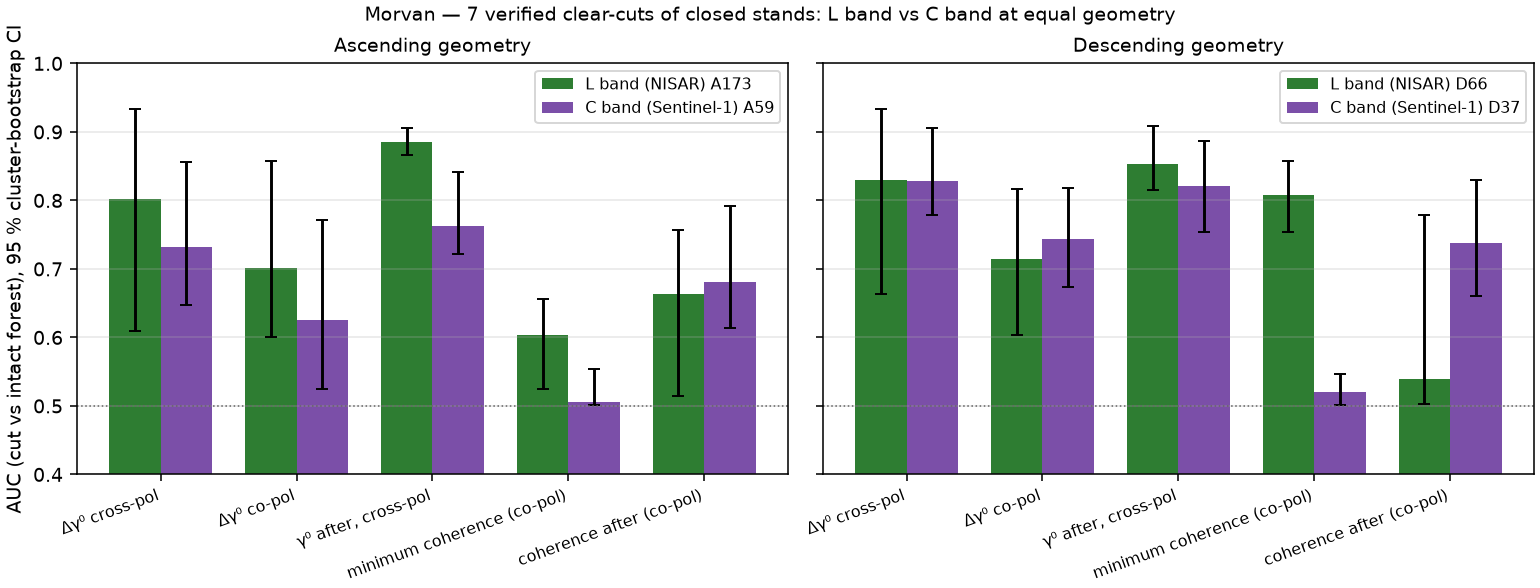
\includegraphics[width=0.92\linewidth, height=0.50\textheight, keepaspectratio]{m8_summary_L_vs_C.png}
	\vspace{-4pt}
	\captionof{figure}{AUC coupe / forêt intacte des cinq indicateurs, 7 coupes de peuplement (IC 95~\%).}

	\vspace{-4pt}
	\keynum{Lband}{0,80 / 0,83}{$\Delta\gamma^0$ croisée \Lb{L}\\montante / descendante}\hfill
	\keynum{Cband}{0,73 / 0,83}{$\Delta\gamma^0$ croisée \Cb{C}\\montante / descendante}\hfill
	\keynum{myblue}{d = 2,1 / 1,6}{contraste plus fort en \Lb{L}\\(d de Cohen, descendante)}
\end{frame}

\begin{frame}{\phantom{x}}
	\frametitle{Résultats et discussion (2/6)}
	\slidesubtitle{2-La forêt reste cohérente en bande L, pas en bande C}
	\begin{columns}[c]
		\column{0.50\textwidth}
		\centering\scriptsize
		\renewcommand{\arraystretch}{1.25}
		\begin{tabular}{|l|c|c|}
			\hline
			\rowcolor{myblue}\textcolor{white}{\textbf{Géométrie}} & \textcolor{white}{\textbf{Forêt intacte}} &
			\textcolor{white}{\textbf{AUC coh. min.}} \\
			\hline
			\Lb{L A173} & 0,35 -- 0,70 & 0,60 \\
			\Lb{L D66} & 0,48 -- 0,71 & \textbf{0,81} \\
			\Cb{C A59} & 0,30 -- 0,36 & 0,51 \\
			\Cb{C D37} & 0,25 -- 0,27 & 0,52 \\
			\hline
		\end{tabular}
		\captionof{table}{Cohérence médiane à 12~j et séparation des coupes.}

		\column{0.48\textwidth}
		\footnotesize
		\begin{itemize}
			\setlength{\itemsep}{4pt}
			\item \textbf{H1 confirmée} : en \Cb{C}, la forêt est au plancher de l'estimateur, comme dans les Vosges
			\item \Lb{D66} : paire 29/08 $\to$ 10/09, \textbf{0,45} sur les coupes contre \textbf{0,63} en forêt
			\item \Lb{A173} : deux paires de fin août décorrèlent \textbf{toute} la forêt (0,35) ; pluie ou vent
			probable, non vérifié
			\item En \Cb{C}, la coupe ne se voit qu'\emph{après} : le sol nu redevient un peu cohérent (jusqu'à 0,53),
			4 à 8 semaines plus tard
		\end{itemize}
	\end{columns}
\end{frame}

\begin{frame}{\phantom{x}}
	\frametitle{Résultats et discussion (3/6)}
	\slidesubtitle{3-La méthode du guide transposée au radar}
	\vspace{-4pt}
	\centering
	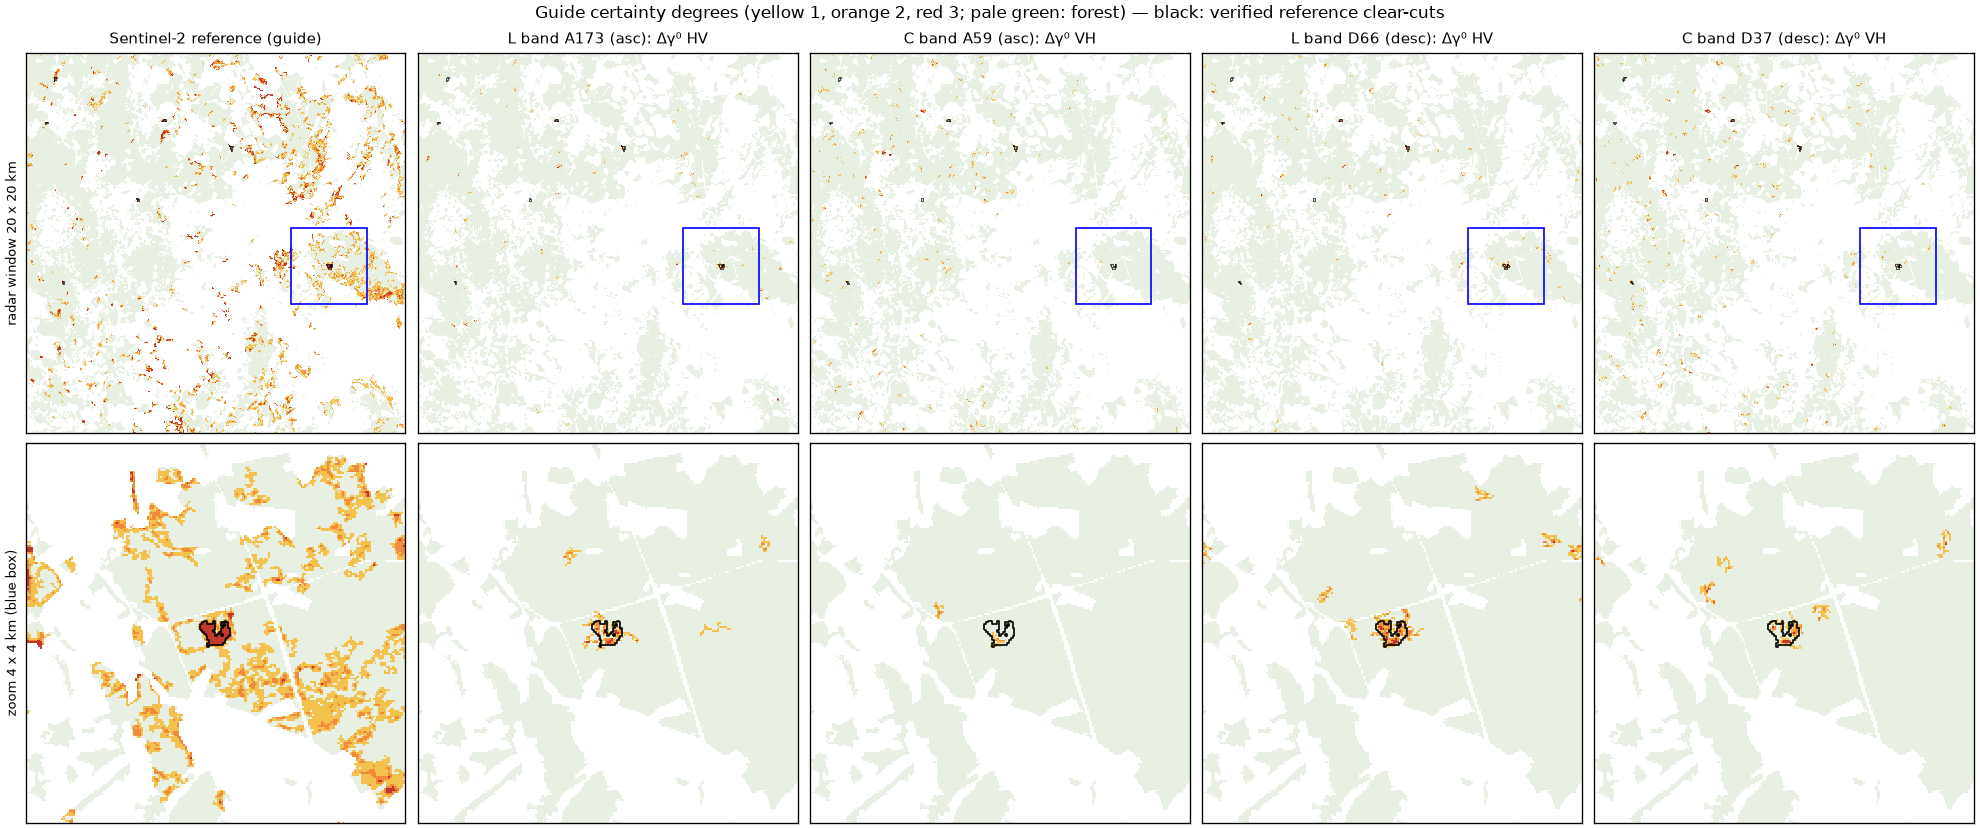
\includegraphics[width=\linewidth, height=0.42\textheight, keepaspectratio]{m6_guide_maps.png}
	\vspace{-6pt}
	\captionof{figure}{Degrés du guide sur $\Delta\gamma^0$ croisée ; en bas, zoom de $4\times4$~km.}

	\vspace{-4pt}
	\scriptsize
	\renewcommand{\arraystretch}{1.15}
	\begin{tabular}{|l|c|c|c|c|c|}
		\hline
		\rowcolor{myblue}\textcolor{white}{\textbf{Géométrie}} & \textcolor{white}{\textbf{Omission}} &
		\textcolor{white}{\textbf{Commission}} & \textcolor{white}{\textbf{Kappa}} &
		\textcolor{white}{\textbf{Coupes trouvées}} & \textcolor{white}{\textbf{Fausses alertes}} \\
		\hline
		\Lb{L A173} / \Lb{L D66} & 55 / 51~\% & 62 / 64~\% & \textbf{0,41 / 0,41} & \textbf{5/7} & 11--13~ha \\
		\Cb{C A59} / \Cb{C D37} & 83 / 84~\% & 94 / 83~\% & 0,08 / 0,16 & 3/7 -- 2/7 & 41--52~ha (degré 2) \\
		\hline
	\end{tabular}
\end{frame}

\begin{frame}{\phantom{x}}
	\frametitle{Résultats et discussion (4/6)}
	\slidesubtitle{4-Pourquoi le guide favorise la bande L, et ce que sont les fausses alertes}
	\begin{columns}[T]
		\column{0.48\textwidth}
		\begin{block}{AUC égale, kappa différent}
			\footnotesize
			\begin{itemize}
				\setlength{\itemsep}{3pt}
				\item L'\textbf{AUC} mesure le classement moyen des pixels
				\item Le guide ne garde que la \textbf{queue} de la distribution ($m-2\sigma$, $m-3\sigma$)
				\item Là, c'est l'écart en écarts-types qui compte : d = \Lb{2,13} contre \Cb{1,63}
				\item Résultat stable pour les \textbf{4 références} (kappa \Lb{L} 0,13--0,41 ; \Cb{C} 0,04--0,19)
			\end{itemize}
		\end{block}

		\column{0.48\textwidth}
		\begin{block}{Audit des 15 plus grandes fausses alertes}
			\footnotesize
			\begin{itemize}
				\setlength{\itemsep}{3pt}
				\item \Lb{NISAR D66} : \textbf{2 coupes tardives} probables (après la fenêtre S2), 13 sénescences,
				lisières, mélèzes jaunis
				\item \Cb{S1 D37} : \textbf{aucune coupe} ; \textbf{8/15} sur des parcelles \textbf{déjà ouvertes}
				en juin (anciennes coupes, landes)
			\end{itemize}
		\end{block}
		\vspace{2pt}
		\footnotesize \Lb{L} répond à la perte des \textbf{troncs}, \Cb{C} à tout changement de la
		\textbf{strate basse}.
	\end{columns}
\end{frame}

\begin{frame}{\phantom{x}}
	\frametitle{Résultats et discussion (5/6)}
	\slidesubtitle{5-Datation des coupes et poids de la référence}
	\begin{columns}[c]
		\column{0.58\textwidth}
		\centering
		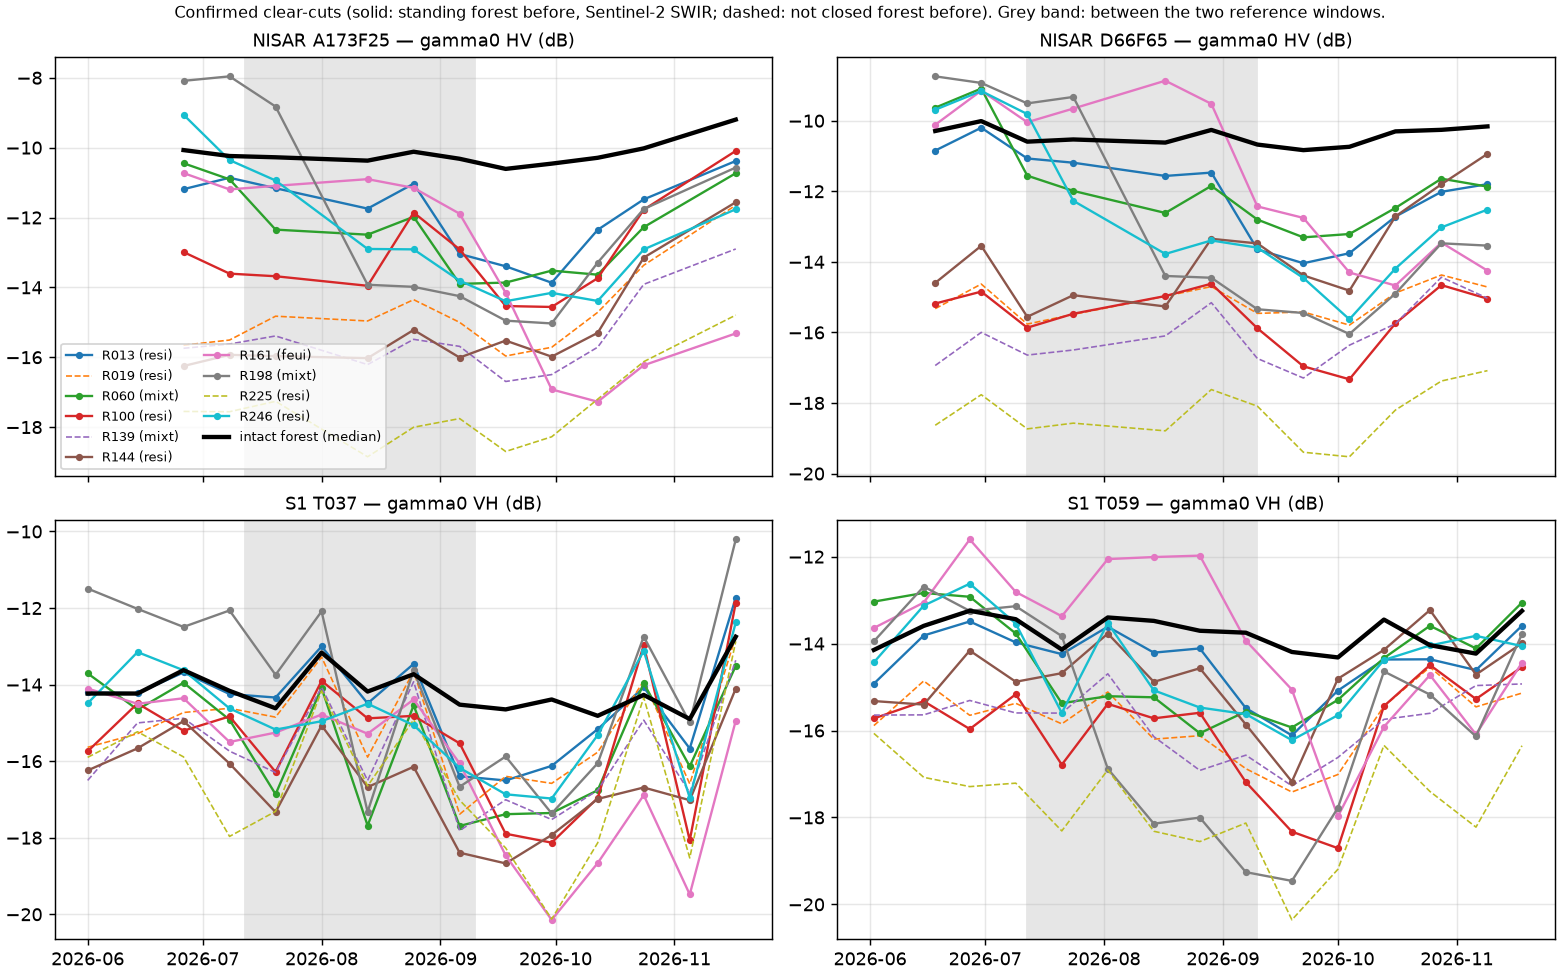
\includegraphics[width=\linewidth, height=0.62\textheight, keepaspectratio]{m7_cut_timeseries.png}
		\vspace{-4pt}
		\captionof{figure}{$\gamma^0$ croisée des coupes et de la forêt intacte (trait noir).}

		\column{0.40\textwidth}
		\footnotesize
		\begin{itemize}
			\setlength{\itemsep}{3pt}
			\item \Lb{L} : séries lisses, \textbf{dates concordantes} entre A173 et D66
			\item \Cb{C D37} : sauts synchrones de $\pm3$~dB (humidité) ; 5 coupes sur 7 dans la même paire
			\item \Cb{C A59} resserre R198 (21/07--02/08)
		\end{itemize}
		\vspace{2pt}
		\scriptsize
		\renewcommand{\arraystretch}{1.15}
		\begin{tabular}{|l|c|c|}
			\hline
			\rowcolor{myblue}\textcolor{white}{\textbf{Référence}} & \textcolor{white}{\textbf{\Lb{L}}} &
			\textcolor{white}{\textbf{\Cb{C}}} \\
			\hline
			auto (60) & 0,56 & 0,51--0,53 \\
			peuplement (7) & 0,80--0,83 & 0,73--0,83 \\
			\hline
		\end{tabular}

		\vspace{2pt}
		\footnotesize\textcolor{myorange}{\textbf{La référence domine tout}} : sans photo-interprétation,
		aucune bande ne \enquote{voit} les coupes.
	\end{columns}
\end{frame}

\begin{frame}{\phantom{x}}
	\frametitle{Résultats et discussion (6/6)}
	\slidesubtitle{6-Bilan des hypothèses et comparaison avec les Vosges}
	\centering
	\renewcommand{\arraystretch}{1.3}
	\setlength{\tabcolsep}{4pt}
	\footnotesize
	\begin{tabular}{|c|p{5.2cm}|p{5.0cm}|c|}
		\hline
		\rowcolor{myblue}\textcolor{white}{\textbf{H}} & \textcolor{white}{\textbf{Morvan (7 coupes)}} &
		\textcolor{white}{\textbf{Vosges (1 coupe)}} & \textcolor{white}{\textbf{Verdict}} \\
		\hline
		H1 & forêt 0,5--0,7 (L) / 0,25--0,36 (C) & 0,64--0,70 (L) / 0,28 (C) & \textcolor{mygreen}{\textbf{confirmée}} \\
		\hline
		H2 & D66 : 0,81 contre 0,52 ; A173 : 0,60 & 0,91--0,995 contre 0,74 & \textcolor{myorange}{\textbf{partielle}} \\
		\hline
		H3 & d 1,9--2,1 (L) contre 1,0--1,6 (C) ; AUC L $\geq$ C & avantage L en montante seulement &
		\textcolor{myorange}{\textbf{partielle}} \\
		\hline
		H4 & croisée $>$ co-pol., 4 géométries sur 4 & HV $\geq$ HH & \textcolor{mygreen}{\textbf{confirmée}} \\
		\hline
	\end{tabular}

	\vspace{0.8em}
	\begin{alertblock}{Message scientifique}
		\small Deux sites, même message : l'avantage net de la bande L est \textbf{interférométrique}. En
		rétrodiffusion, les AUC sont proches, mais le \textbf{contraste} plus fort de la bande L rend la méthode
		opérationnelle du guide nettement plus efficace.
	\end{alertblock}
\end{frame}

% ================================================================
\section{Regard critique}
% ================================================================

\begin{frame}{\phantom{x}}
	\frametitle{Regard critique}
	\vspace{-4pt}\slidesubtitle{Forces et limites de la démarche}
	\small
	\begin{columns}[T]
		\column{0.48\textwidth}
		\begin{exampleblock}{Forces}
			\footnotesize
			\begin{itemize}
				\setlength{\itemsep}{1pt}
				\item Méthode opérationnelle reconnue (guide de l'Irstea), appliquée puis \textbf{critiquée}
				\item Référence vérifiée coupe par coupe, test \enquote{forêt avant} indépendant
				\item Géométrie égale dans les deux directions
				\item Contrôle avant coupe, 4 références, érosion de 20~m : ordre L / C stable
				\item Audit des fausses alertes des deux bandes
				\item Chaîne reproductible, configuration par site
			\end{itemize}
		\end{exampleblock}

		\column{0.48\textwidth}
		\begin{alertblock}{Limites}
			\footnotesize
			\begin{itemize}
				\setlength{\itemsep}{1pt}
				\item \textbf{7 coupes, 15~ha} : IC larges, différences d'AUC non significatives
				\item Une saison, un paysage dominé par les résineux
				\item Référence optique : coupes tardives et sans sol nu manquées
				\item Estimateurs de cohérence différents ; produits NISAR provisoires
				\item Météo non vérifiée (décorrélation de fin août)
				\item Objectif du guide (10~\%) non atteint
			\end{itemize}
		\end{alertblock}
	\end{columns}
\end{frame}

% ================================================================
\section{Conclusion et perspectives}
% ================================================================

\begin{frame}{\phantom{x}}
	\frametitle{Conclusion et perspectives}
	\vspace{-6pt}\small
	\begin{columns}[T]
		\column{0.50\textwidth}
		\begin{block}{Conclusions}
			\footnotesize
			\begin{enumerate}
				\setlength{\itemsep}{3pt}
				\item \textbf{H1 confirmée sur un 2\textsuperscript{e} site} : la forêt reste cohérente en \Lb{L}, pas en \Cb{C}
				\item \textbf{Cohérence L} : AUC 0,81 en descendante, mais sensible aux épisodes de décorrélation
				\item \textbf{Guide au radar} : kappa \Lb{0,41} (5/7 coupes) contre \Cb{0,08--0,16}
				\item \textbf{Complémentarité} : \Cb{C} réagit à la strate basse, \Lb{L} aux troncs
				\item \textbf{Référence} : la photo-interprétation est indispensable
			\end{enumerate}
		\end{block}

		\column{0.46\textwidth}
		\begin{block}{Perspectives pour le stage}
			\scriptsize
			\begin{itemize}
				\setlength{\itemsep}{1pt}
				\item \textbf{Détecteur} combinant cohérence L, $\gamma^0$ L et revisite C, avec confirmation
				temporelle
				\item \textbf{Plusieurs saisons} et régions ; référence par images à un an d'écart (comme le guide)
				\item Seuils du guide \textbf{adaptés} à la phénologie
				\item Données météo pour expliquer les décorrélations
				\item \textbf{ROSE-L} et \textbf{ISCE3} \parencite{esa2020rosel,isce3} ; glissements sous forêt en InSAR L
			\end{itemize}
		\end{block}
	\end{columns}
\end{frame}

\begin{frame}
	\vfill
	\centering
	{\Large Merci pour votre attention !}

	\vspace{1em}
	\small\textcolor{mydgray}{Deux sites, même message : la bande L garde la forêt \emph{cohérente}, et une coupe y
		devient un \emph{événement}.}
	\vfill
\end{frame}

% ================================================================
\appendix
% ================================================================

\begin{frame}[fragile]{Annexe : reproduction}
	\scriptsize
\begin{verbatim}
python scripts/morvan/m1_ign.py              # contour G23, BD Forêt
python scripts/morvan/m2_s2_guide.py         # guide sur Sentinel-2
python scripts/morvan/m2b_photo_check.py     # photo-interprétation
python scripts/morvan/m2c_forest_before.py   # test forêt avant
python scripts/morvan/m3_radar_window.py     # fenêtre radar
python scripts/morvan/m4_fetch_nisar.py      # NISAR à distance
python scripts/morvan/m4_fetch_s1.py         # Sentinel-1 réduits
python scripts/morvan/m5_process_s1.py --orbit 59   # SNAP (et 37)
python scripts/morvan/m6_compare.py          # + --ref ... --tag ...
python scripts/morvan/m6b_commission_audit.py --geom S1_T037 --var d_g0_VH
python scripts/morvan/m6c_coherence_pairs.py
python scripts/morvan/m7_dating.py
python scripts/morvan/m8_make_tables.py
\end{verbatim}
	\normalsize Rapports complets (FR et EN) : \texttt{reports/morvan/latex/}.
\end{frame}

\begin{frame}{Annexe : audit des fausses alertes Sentinel-1}
	\centering
	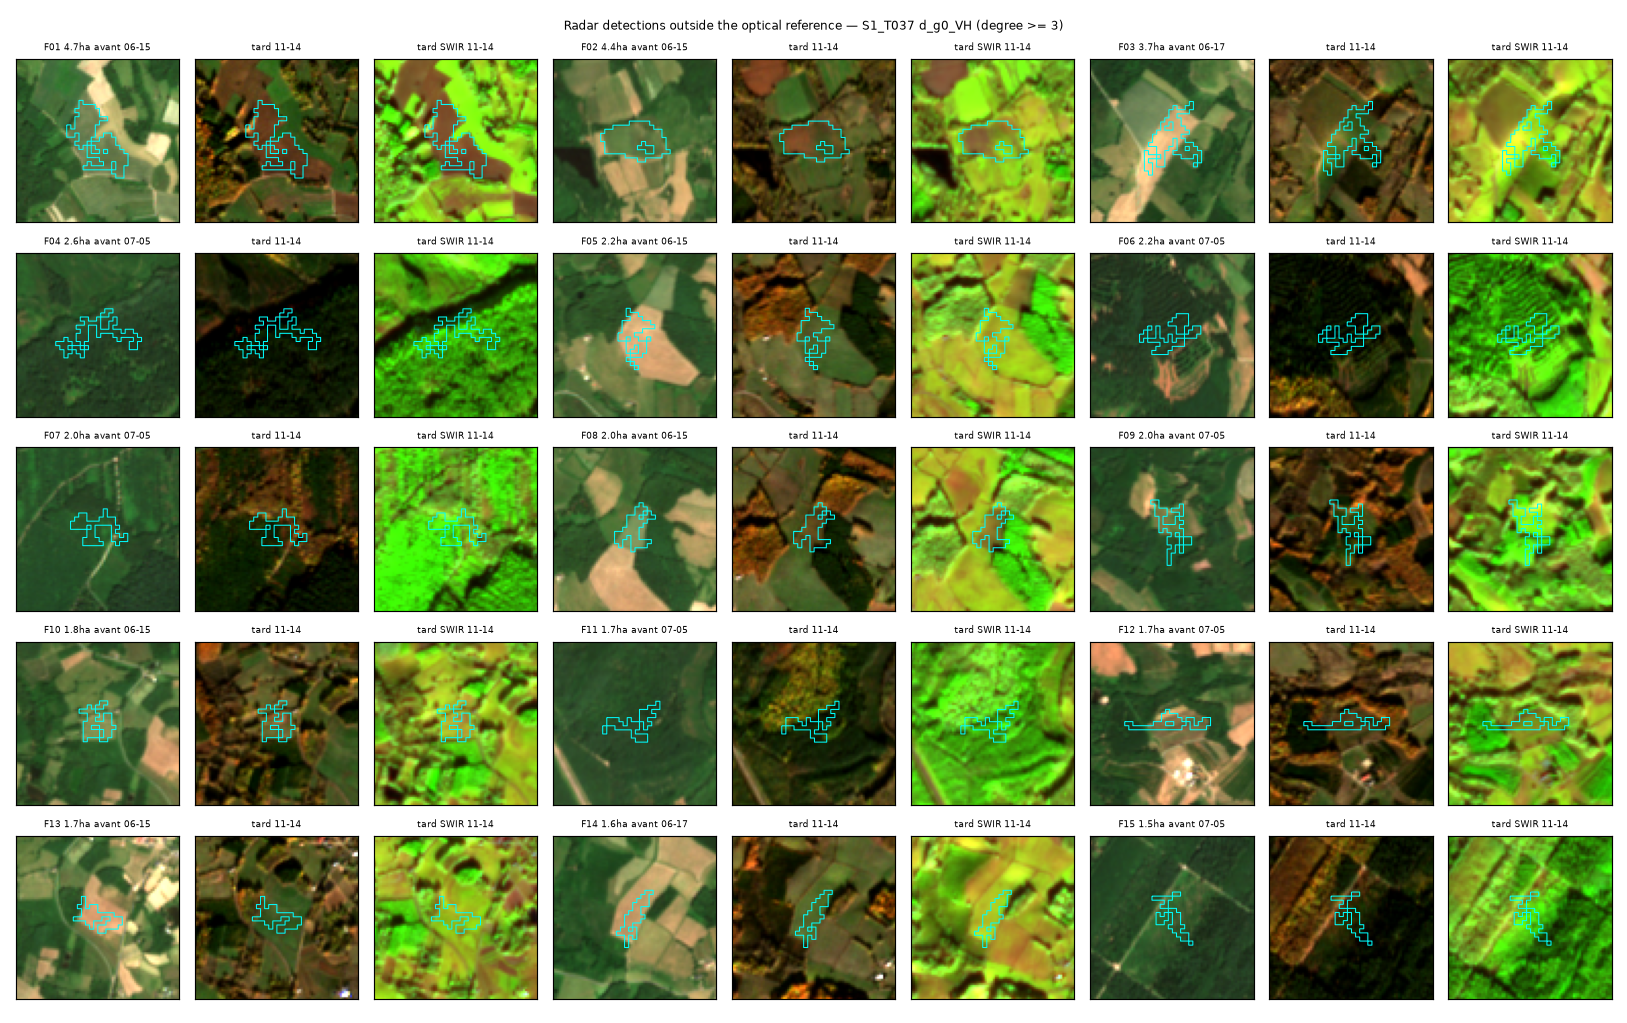
\includegraphics[height=0.82\textheight, width=\linewidth, keepaspectratio]{m6b_commission_S1_T037_d_g0_VH.png}
\end{frame}

\begin{frame}[allowframebreaks]{Références}
	\scriptsize
	\printbibliography[heading=none]
\end{frame}

\end{document}
